\begin{comment}
	\pagebreak
\end{comment}

\section{Fully Convolutional Neural Network}
\begin{comment}
	The main difference to classical CNN is that we don't want to only work with fixed sized images as input. 
	This limitation comes from the fully connected layers in the end.\\
\end{comment}

\textbf{Goal:} Pixel-to-pixel classification
\begin{comment}
	By removing the size constraints of the input pictures allows us to classify pixels by using their local neighbourhood.\\
	\textbf{Drawback:} We don't get the information of the whole context.\\
	The basic approach is using a standard CNN to learn features of the input image (encoding), which is followed by a decoder who projects the learned features to the higher resolution pixel space.\\
	\begin{Figure}
 		\centering
 		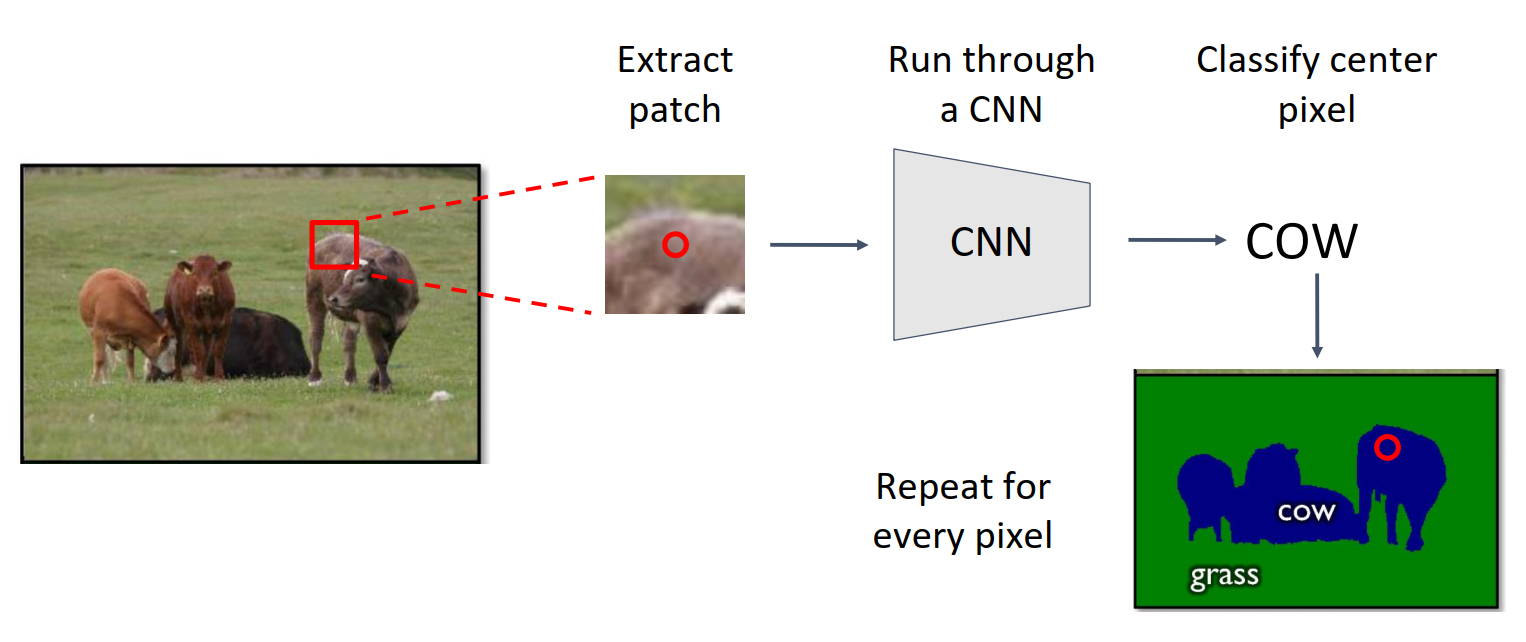
\includegraphics[width=\linewidth]{graphic/fcnn-semantic-segmentation-pipeline}
 		\captionof{figure}{Pixel-wise classification pipeline}
	\end{Figure}
\end{comment}

\textbf{Low-res:} due to all the pooling and down-sampling\\
\begin{comment}
	This results in low resolution and fuzzy object boundaries.
	Newer architectures can mitigate this by upsampling again.\\
	The learned features on each downsampled level are copied to the upsampling (decoding) stream, to give the fcnn a chance to include features of different levels.\\ 
	
	\begin{Figure}
 		\centering
 		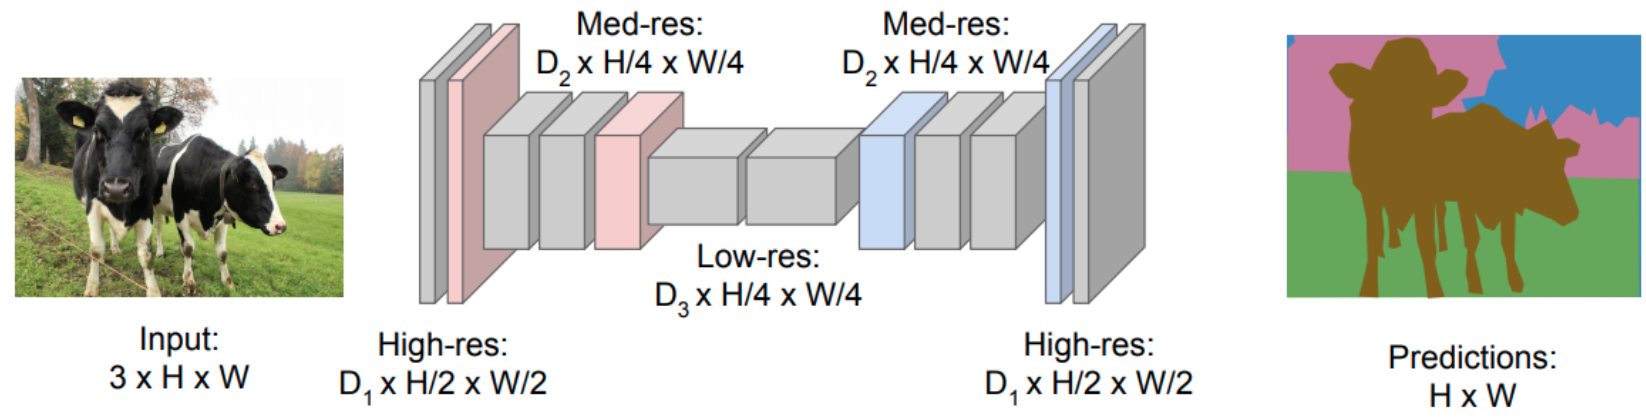
\includegraphics[width=\linewidth]{graphic/fcnn-low-res-mitigation}
 		\captionof{figure}{Downsample and than upsample to increase resolution again}
	\end{Figure}
\end{comment}

\textbf{Upsampling (NN):} copy value for the whole output\\ 
\begin{comment}
	Upsampling can be seen as interpolation, increasing the resolution of the signal.\\
	
	\begin{Figure}
 		\centering
 		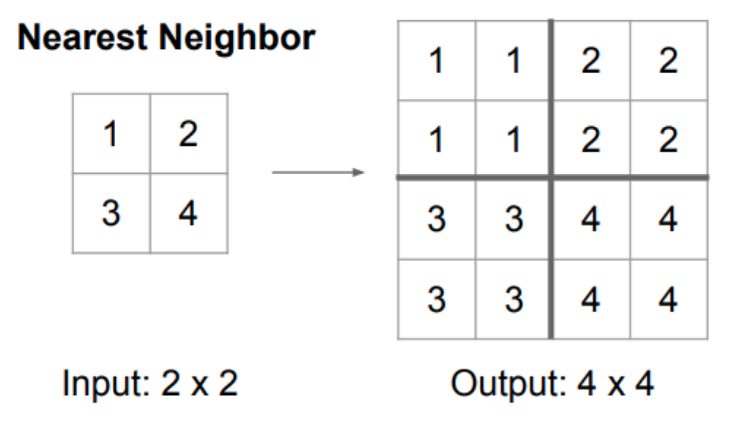
\includegraphics[width=\linewidth]{graphic/fcnn-nn-upsampling}
 		\captionof{figure}{Copy input pixel to all output pixels}
	\end{Figure}
\end{comment}

\textbf{Bed-of-nails:} zero all outputs but one copy of input
\begin{comment}
	\begin{Figure}
 		\centering
 		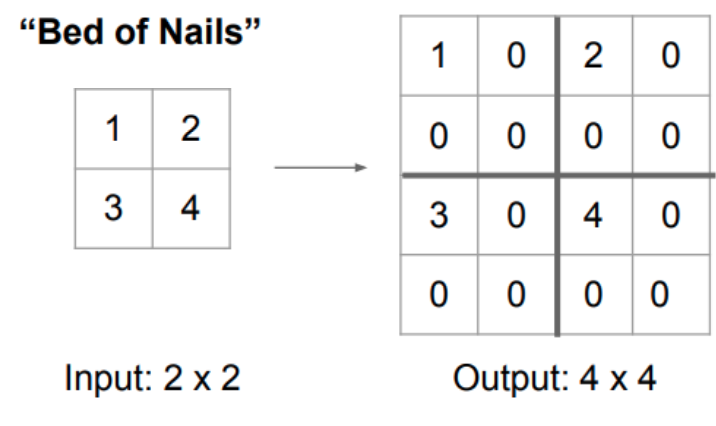
\includegraphics[width=\linewidth]{graphic/fcnn-bos-upsampling}
 		\captionof{figure}{Copy input pixel to one output pixels, rest zero}
	\end{Figure}
\end{comment}

\textbf{Max-Unpooling:} remember max pooling, BOF to that location\\
\begin{comment}
	\begin{Figure}
 		\centering
 		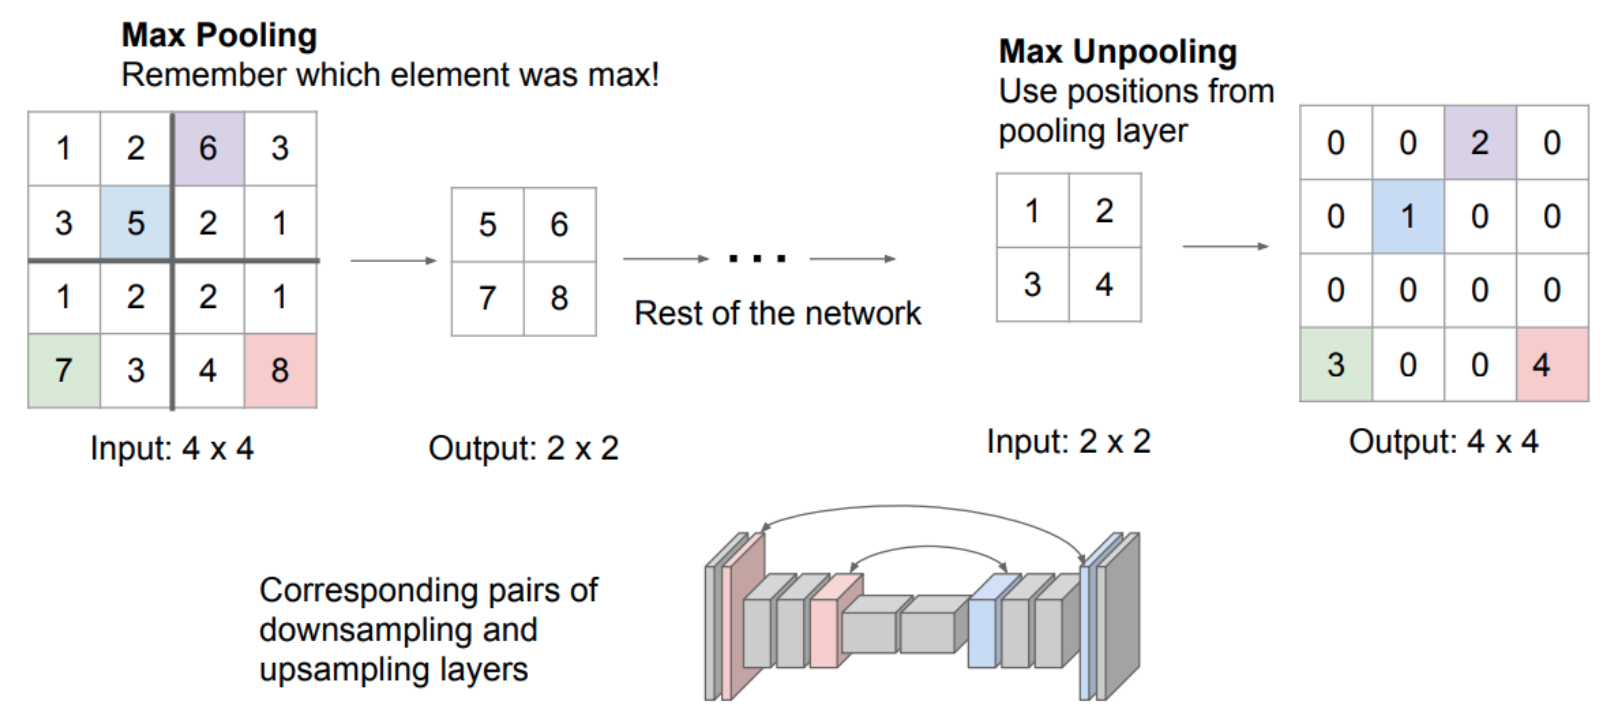
\includegraphics[width=\linewidth]{graphic/fcnn-max-unpooling-upsampling}
 		\captionof{figure}{Copy input pixel to location of the max pooling pixel}
	\end{Figure}
\end{comment}

\textbf{Transpose Conv:} input gives (learnable) weight for filter\\
\begin{comment}
	\begin{Figure}
 		\centering
 		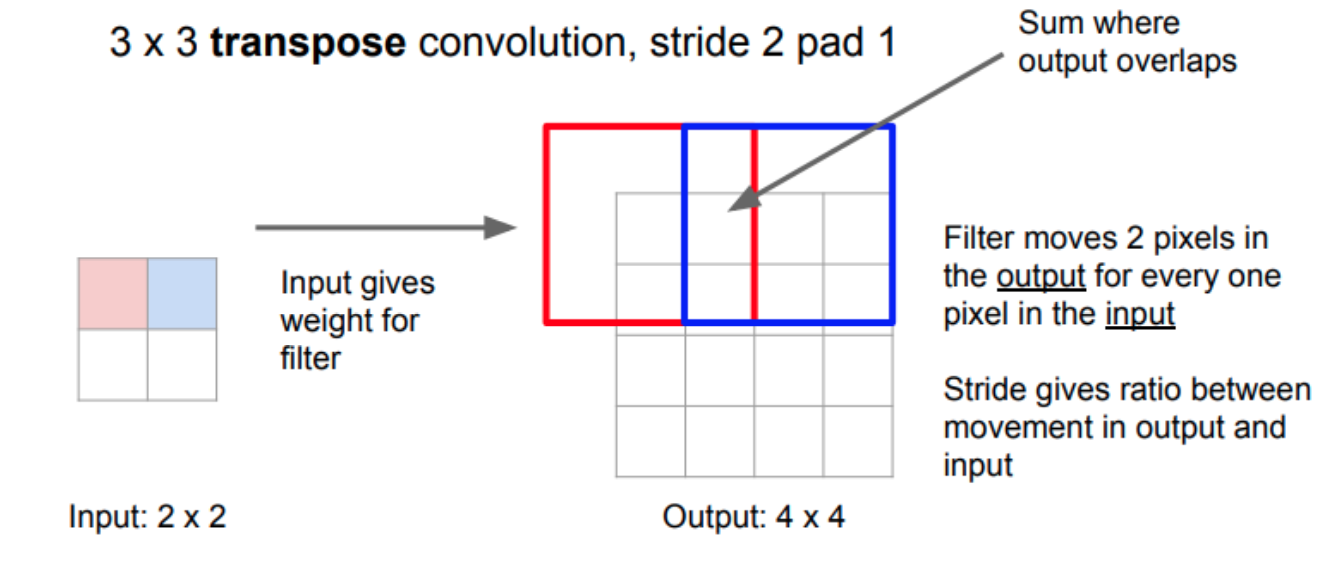
\includegraphics[width=\linewidth]{graphic/fcnn-transpose-convolution}
 		\captionof{figure}{Input pixel gives the weight for a filter}
	\end{Figure}
\end{comment}

\textbf{UNet:} TransCov + Skip connections\\
\begin{comment}
	Main idea: combine global and local feature maps by copying corresponding tensors from earlier stages.\\
	Also, the downsampling information is pretty shallow, upsampling performance is improved when including "pre-downsamplin" information.\\

	\begin{Figure}
 		\centering
 		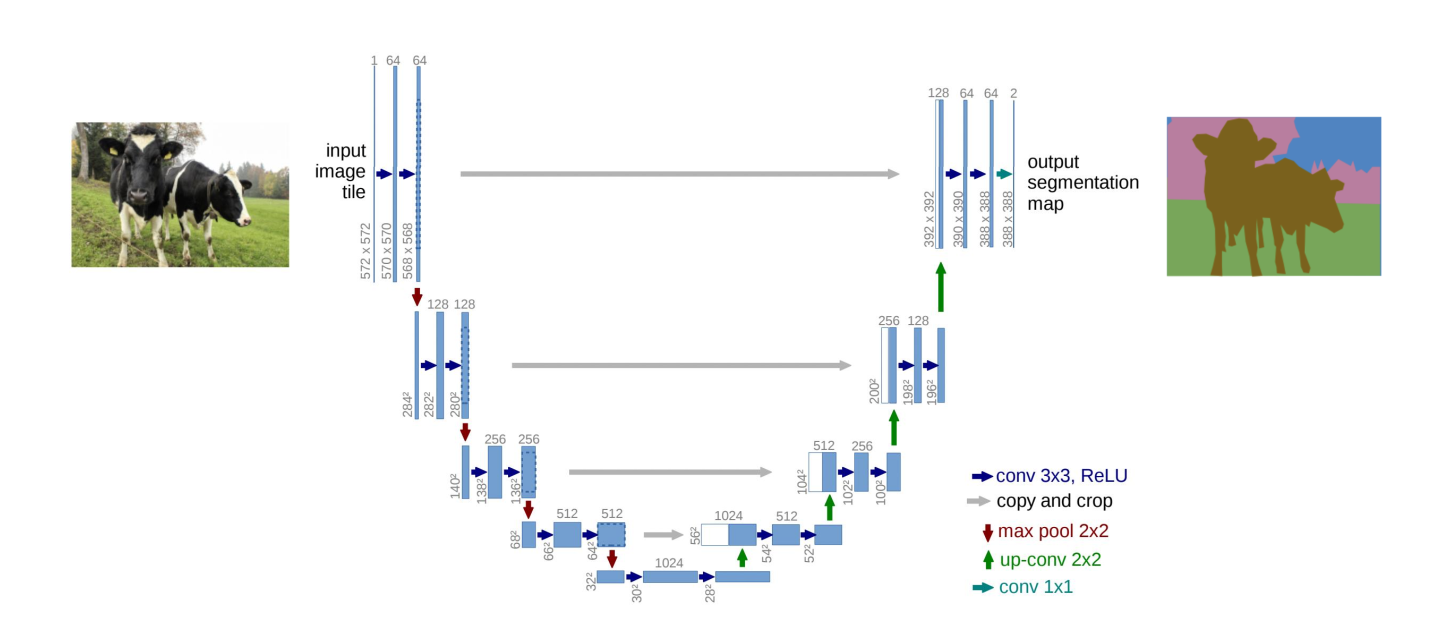
\includegraphics[width=\linewidth]{graphic/fcnn-unet}
 		\captionof{figure}{U-Net architecture}
	\end{Figure}
\end{comment}





